

\section{Outline of our approach}
\label{s:outline}
%We now give an outline of our approach %using a bank account example,   where funds may be transferred between accounts only if the account's password has been supplied.
%\sophiaPonder[more succinct]{expanding on the bank example from earlier.}


 \subsection{Bank Account -- three modules}
\label{s:bank}
  
Module \ModA consists of an empty 
\prg{Password} class, and an  \prg{Account} class with a password, and a balance, an \prg{init} method to 
initialize the password, and 
a
\prg{transfer} method. \sophiaPonder[chopped "where each instance models a unique password", because NOT TRUE!!]{}
%
% (Note that we assume private fields are accessible ``class-wide''.)
%
% (methods may read and write fields of any instance of a class)
%
%and that passwords are unforgeable and not enumerable (again as
%in Java, albeit without reflection).
%
% 
\begin{lstlisting}[mathescape=true, language=Chainmail, frame=lines]
module $\ModA$
  class Account
    field balance:int 
    field pwd: Password
    method transfer(dest:Account, pwd':Password) -> void
      if this.pwd==pwd'
        this.balance-=100
        dest.balance+=100
     method init(pwd:Pasword) -> void
      if this.pwd==null
        this.pwd=pwd'
  class Password
\end{lstlisting}
%
\noindent 
We can capture the intended
semantics of  
\prg{transfer}  
through \susan[]{a}  ``classical''
specification with pre- and postconditions as \emph{e.g.,} in \cite{Leavens-etal07,dafny13},
with ``explicit framing'' --   
 \sophiaPonder[our term?]{rather than \prg{modifies} we give assertions   about preservation of values.}
 \sophiaPonder[We also need to say where we use that -- later on]{}
%\sophiaPonder[]{
%-- note that we always treat all free variables as universally quantified.
%}
\ModA's implementation of the \prg{transfer} method meets
this specification.



\begin{lstlisting}[mathescape=true, frame=lines, language=Chainmail]
$\Sclassic$  $\triangleq$
   method transfer(dest:Account, pwd':Password) -> void {
       ( PRE:  this.balance=bal1 $\wedge$ this.pwd==pwd' $\wedge$ dest.balance=bal2 $\wedge$ dest=/=this 
         POST: this.balance == bal1-100 $\wedge$  dest.balance == bal2+100 )
       ( PRE: this.balance=bal1 $\wedge$ this.pwd=/=pwd' $\wedge$ dest.balance=bal2
         POST: this.balance == bal1 $\wedge$  dest.balance=bal2 )
       ( PRE: a : Account $\wedge$ a=/=this $\wedge$ a=/=dest  $\wedge$ a.balance=bal $\wedge$ a.pwd=pwd1
         POST:  a.balance=bal $\wedge$ a.pwd=pwd1)
       ( PRE: a : Account $\wedge$ a.pwd=pwd1  
         POST: a.pwd=pwd1)       
\end{lstlisting}
%\footnote{Perhaps omit some of the lines here, but we do need them all in the full discussion}
 
 

Now consider the following alternative implementations:
\ModB allows any client to reset an account's password at any time, while
\ModC requires the existing password in order to change it.

%% The method \prg{transfer} in all three versions of the class \prg{Account} satisfies the (ClassicSpec), 
%% however, while executing the first and third version of \prg{Account} won't exhibit unwanted behaviour, the second version doesn't preclude it.
%Namely version II allows any client to change the password of the
%account, and then to repeatedly withdraw money from it.

  
% On the other hand, we expect our software -- even if complex -- to provide some simple, high level
%guarantees, e.g. email addressed to me personally will not be read by a third party unless I explicitly 
%forwarded it to them.
%We except  our software to  behave correctly, even when used by a careless or malicious third party. 
%Such use of a software often consist of a sequence of actions performed on the module. 
%
%Software components respond to single actions, 
%or to sequences of such single actions. 
%When thinking about a software component we want think about the behaviour of each 
%action in isolation, but also about the \emph{emergent behaviour}, ie all
% the possible effects of the combinations of these actions. 
  
  

\begin{tabular}{lll}
\begin{minipage}[b]{0.42\textwidth}
\begin{lstlisting}[mathescape=true, language=chainmail, frame=lines]
module $\ModB$
  class Account
    field balance:int 
    field pwd: Password 
    method transfer(..) ...
      ... as earlier ...
    method init(...) ...
       ... as earlier ...
    method set(pwd': Password)
      this.pwd=pwd'
      
  class Password
\end{lstlisting}
\end{minipage}
&\ \ \  \ \   &%
\begin{minipage}[b]{0.45\textwidth}
\begin{lstlisting}[mathescape=true, language=chainmail, frame=lines]
module $\ModC$
  class Account
    field balance:int 
    field pwd: Password 
    method transfer(..) 
      ... as earlier ...
    
    
    method set(pwd',pwd'': Password)
      if (this.pwd==pwd') 
        this.pwd=pwd''
  class Password
\end{lstlisting}
\end{minipage} 
\end{tabular}

Although the \prg{transfer} method is the same in
all three alternatives, and each one satisfies \Sclassic,
code \sophiaPonder[this this needs space, hence line break]{such as}
\\ 
$\ \strut \hspace{.2in} $ \prg{an\_account.set(42); an\_account.transfer(42,rogue\_account)}
\\ 
is enough to drain  \prg{an\_account} in \ModB without knowing the password.


 \subsection{Bank Account -- the right specification}
\label{s:bankSpecEx}

We need \sophiaPonder[is that clear?]{a specification with which to} rule out \ModB while permitting \ModA and
\ModC. The catch is that the vulnerability present in \ModB is the result
of  \emph{emergent} behaviour from the interactions of the \prg{set}
and \prg{transfer} methods --- even though \ModC also has a
\prg{set} method, it does not exhibit the unwanted interaction.
This is exactly where a necessary condition can help:
we want to avoid transferring money
(or more generally, reducing an account's balance)
\textit{without} the existing account password.  Phrasing the same condition
the other way around % gives us a positive statement that still
rules out the theft: that money \textit{can only} be
transferred when the account's password is known.


In \Nec  syntax, and \sd{recalling section \ref{intro:this:work}, }
 

%
%% The flaw in version {\sf{II}} arises from 
%% can be used to overwrite the
%% password, and then using the new password \prg{transfer}  can be called.
% If we want the \prg{Account} class to be robust, we must prohibit the password from being freely available.
%
%
%% In this paper, we show how \textit{necessity specifications} can solve
%% this progkem.  
%%  Therefore, we propose a %holistic 
%%  specification which says that
%%  the \prg{balance} of an \prg{Account} reduces only if an object which does not belong to the
%%  module has access to the password:
%
%
 %% Therefore, we propose a %holistic 
 %% specification which says that
 %% the \prg{balance} of an \prg{Account} reduces only if an object which does not belong to the
 %% module has access to the password:
%
\begin{lstlisting}[language = Chainmail, mathescape=true, frame=lines]
   $\text{\SrobustA}$  $\triangleq$   from   a:Account $\wedge$ a.balance==bal    next    a.balance < bal
                onlyIf $\exists$ o,a'. [$\external{\texttt{o}}$ $\wedge$ $\calls{\texttt{o}}{\texttt{a}}{\texttt{transfer}}{\texttt{a.pwd},\texttt{a'}} $]    
                
   $\text{\SrobustB}$  $\triangleq$   from   a:Account $\wedge$ a.balance==bal    to    a.balance < bal
                onlyIf $\exists$ o.[$\external{\texttt{o}}$ $\wedge$ $\access{\texttt{o}}{\texttt{a.pwd}}$]    
           
\end{lstlisting}
%
%
% 
%% In more detail, the specification from above says that if in the current
%% configuration \prg{a} is an \prg{Account},
%% and in some future configuration \prg{a} will have a balance less than the current one, then,in the \emph{current} configuration
%% there must exist some object \prg{o}, which is \emph{external} to our module (does not belong to module
 %% \prg{AccountMdl}), and which has access to \prg{a}'s password.
 %
%% T9hu having access to the password is a necessary condition for the balance to reduce.

\sd{Indeed, all three modules   satisfy  \SrobustA;  this demonstrates that \SrobustA is not
strong enough. On the other hand, \ModA and \ModC satisfy \SrobustB, while \ModB does not.  }

A critical point of \SrobustB % this \Nec specification 
is that it is
expressed in terms of observable effects (the account's balance is
reduced: \prg{a.balance < bal}) and the shape of the heap 
(external access to the password:
$\external{\prg{o}}\ \wedge\ \access{\prg{o}}{\prg{a.pwd}}$) 
rather than in terms of individual methods such as
\prg{set} and \prg{transfer}.
This gives our specifications the
vital advantage that they can be used to constrain
\textit{implementation} of a bank account with a balance and a
password, irrespective of the API it
offers, the services it exports, or the dependencies on other parts of
the system.

 This example also demonstrates that 
adherence to   \Nec specifications is not monotonic:
adding a method to a module does not necessarily preserve adherence to
a specification, 
and while separate methods may adhere to a  specification, their combination does
not necessarily do so. 
\sd{For example, \ModA satisfies \SrobustB, while \ModB does not.}
This is why we say that \Nec   specifications capture a module's \emph{emergent behaviour}. 
 

%\jm[TODO: in the proof later we need to mention that there is a difference between the overall proof (no mention of the methods), and the intermediate ones (that do mention the methods)]{}
\subsubsection{How applicable is  \SrobustB?}
\label{sec:how}
Finally, \sd{note that \SrobustB is applicable even though \emph{some} external objects may have access
to the account's password. 
Namely, if the account is passed to a scope which does not know the password, we 
know that its balance is guaranteed not to decrease, even though it may increase. 
}

 
We illustrate this through the following simplified code snippet.
 

\begin{lstlisting}[mathescape=true, language=chainmail, frame=lines]
module $\ModExt$
     ...
    method expecting_payment(untrusted:Object){ 
        a = new Account;
        p = new Password; 
        a.set(null,p);
        ...
        untrusted.make_payment(a);
        ...
    }
}
\end{lstlisting}
 

 The method \prg{expecting\_payment} has as  argument an external object \prg{untrusted}, of unknown provenance.
The method \prg{expecting\_payment} creates a new \prg{Account} and initializes its password. 

Assume that class \prg{Account} is from a module which satisfies \SrobustB. 
Then, 
in the scope of  method \prg{expecting\_payment} external objects have access to the password, 
and the balance may decrease  
during execution of  line 7, or   line \sd{9}. 
\susan[Is this what you want to say? What if the code in line 8 does leak the password?
\sd{I had errors in the lines. The code in line 8 cannot leak the password as it does not have it}]{}
However, if the code in line \sd{7} does not leak the password to \prg{untrusted}, then no external object
in  the scope of the call \prg{make\_payment} at line 8 has access to the password, and then,
even though we are calling   an untrusted object, \SrobustB guarantees that \prg{untrusted}
 will not be able to take any money out of  \prg{a}.
 
\susan[I think this paragraph doesn't add, if anything it has a hostage to fortune. I would just remove it.
\sd{agreed, and removed}]{}
% The purpose of the current paper is being able to express specifications like \SrobustB, and
%and being able to prove adherence. In further work we want to develop logics to leverage such specifications, putting
%informal arguments as the  one of this section onto formal foundations.
 

 
\subsection{Internal and External objects and calls}
\label{s:concepts}

Our work concentrates on guarantees made in an \emph{open} setting; that is, a given module
$M$ must be programmed so that %in such a robust manner
%\sophia[We had agreed no to say "robust", but I think it is OK here. Alternatively, say defensively robust?]{}
execution of $M$ together with \emph{any} \externalM 
module $M'$ will uphold these guarantees. In the tradition of
visible states semantics, we are  only interested in upholding the guarantees while 
$M'$, the  \emph{\externalM} module, is executing. A module can
temporarily break its own invariants,
%%just as a class or monitor can
%%break their invariants,
so long as the broken invariants are never visible externally.
   
We therefore distinguish between \emph{\internalO}
objects --- instances of classes defined in $M$ ---
and \emph{\externalO} objects defined in any other module, and
between \emph{\internalC} calls  (from either an internal or an external object)  made % from \externalO objects
 to \internalO objects and \emph{\externalC} calls made % from \externalC objects
 to \externalC objects. % We are less
% interested in calls made from \internalO objects to \internalO objects, because we only need 
% establish the guarantees when the \externalM module is executing. And we 
%
%
Because we only require guarantees while 
the  \externalM module  is executing,
we develop an \emph{external states} semantics, where
 any internal calls are executed in one, large, step.
With external steps semantics,  the executing object (\prg{this}) is always   external. 
Note that we do not support calls from
\internalO objects to \externalO objects.
 

\newcommand{\vertsp} {\vspace{.05in}} 
 
\subsection{Reasoning about Necessity}
\label{s:approach}

\jm[]{Julian Proposal >>>>>>>>>>>>>>>>>>>>>}

We now give a sketch of the novel concepts we developed in  \Nec logic, 
and how they fit in with existing work in the area.
\jm[]{
\Nec logic consists of 4 components:
\begin{description}
\item[Part 1: Emergent Behavior] \ {is behaviour that arises out 
of any number of steps and interactions with a module interface.}
We infer the \emph{emergent} behaviour out of the conditions of  \sd{several}
single steps. More in \S\ref{s:emergent-proof}.
 \item[Part 2: Single-step conditions] are
 necessary conditions for a given  effect and
a single, \emph{unspecified} step. This step could be an internal call, or any kind of external step.
  % 
    For effects encapsulated by $M$, we can infer such single-step
 conditions by combining the per-method conditions for that effect from 
all   methods in $M$. More in \S\ref{s:module-proof}.
\item[Part 3: Per-method conditions]   % \emph{per-method-condition}, \ie., a 
are  necessary conditions for   given  effect and
  given single, specified, method call. 
To infer these, we  leverage   sufficient conditions 
from classical specifications: % Namely, if 
If the negation of a method's
 classical postcondition implies  a given effect, %the effect we are interested in,
  then the negation of the 
 classical precondition  is a necessary precondition for the effect and the method call. 
More in \S\ref{s:classical-proof}. 
\item[Part 4: Assertion Encapsulation.]  
% \scd{We  introduce the concept} of  \emph{assertion  encapulation}: 
% \scd{We define that an}
An assertion $A$  is
\emph{encapsulated} by  module $M$, if  $A$ can be invalidated only through
 % $M$-\internalC calls. 
calls to methods defined in $M$.
  In other words, a  call to  $M$  is a \emph{necessary} condition for
invalidation of $A$.
Our \Nec logic  is parametric with respect to the 
particular encapsulation
mechanism: here we rely on rudimentary annotations inspired by confinement types
\cite{confined}.
\end{description}
}

\jm[]{These parts are dependent on each other. 
While the above formulation is presented top down,
proofs are built up from the bottom up. Fig. \ref{fig:dependency}
demonstrates the dependencies of the different components of the
proof system.}
\begin{figure}[h]
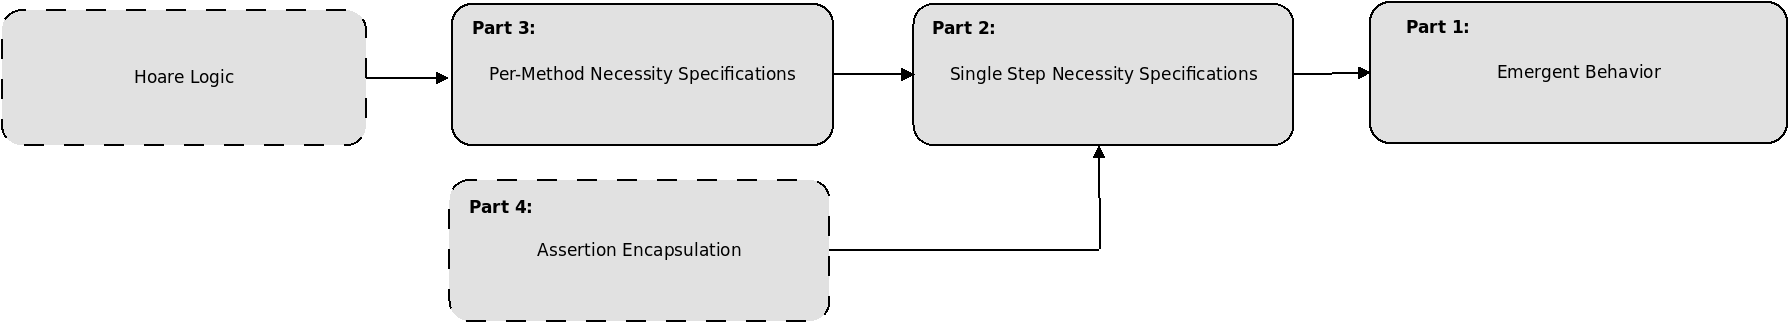
\includegraphics[width=\textwidth]{dependency.png}
   \caption{Components of \Nec Logic \sd{and their Dependencies}
    }
   \label{fig:dependency}
 \end{figure}
 
For illustration, we  outline  a proof that  \ModC adheres to \SrobustB.
 \begin{description}
\item[Part 1: Emergent behaviour] \

\vertsp 

{\fbox{\parbox{\linewidth}{
Our proof of \sd{\ModC's adherence to \SrobustB} %follows
\susan[]{takes} the following steps:
\begin{description}
\item [(A)]
A reduction in an account balance over any number of steps implies that some single intermediate step 
reduced the account's balance.
\item [(B)] 
External knowledge of an account's password is a necessary prerequisite to any single step reducing the balance.
\item [(C)]
An account's password may only be externally known in the future if either
\begin{description}
\item[(C1)]
the password is currently known externally  thus satisfying \SrobustB, or
\item[(C2)] it is possible to coerce the internal module interface to expose the password
\end{description}
\end{description}
The proof of (\textbf{B}) is constructed using \textbf{Part 2} and the proof that (\textbf{C2}) does not hold requires us to use the reasoning in \textbf{Part 2} and \textbf{Part 4}.
}}}

\vertsp 

\item[Part 2: Single-step conditions]  \

\vertsp 

{\fbox{\parbox{\linewidth}{
Our proof of \textbf{(B)} considers single-step conditions, and takes the following form:
\begin{description}
\item[(D)]
An account's balance is an ``encapsulated'' property, that requires module internal computation to change.
\item[(E)]
The only module internal method call that reduces an account's balance is a call to \prg{transfer} with the account's 
password.
\item[(F)]
An external call to \prg{transfer} with an account's password implies that the password is externally known
\end{description}
}}}

\vertsp

{\fbox{\parbox{\linewidth}{
Our proof that \textbf{(C2)} does not hold also considers single-step conditions, and takes the following form:
\begin{description}
\item[(G)]
The internal-only access to an account's password is ``encapsulated'', and required internal computation to invalidate.
\item[(H)]
No internal method call can be used to coerce access to an account's password.
\end{description}
}}}
 
\vertsp
 
 
\item[Part 3: Per-method conditions]   \

\vertsp
{\fbox{\parbox{\linewidth}{
Our proofs of \textbf{(E)} and \textbf{(H)} take the following form:
\begin{description}
\item[(E)] Each method of \ModC (\ie each method in \prg{Account} and \prg{Password}),
if it  causes the  balance to reduce, then the method called was
 \prg{transfer} and the correct password was provided
\item[(H)] Each method of \ModC will not provide external accessibility to the password.
\end{description}
}}}

  
\vertsp


\item[Part 4: Assertion Encapsulation.]  \

\vertsp
{\fbox{\parbox{\linewidth}{
Our proofs of \textbf{(D)} and \textbf{(G)} take the following form:
\begin{description}
\item[(D)] The balance is encapsulated 
by \ModC
\item[(G)] External accessibility to an account's password may 
only be obtained through calls to \ModC -- that is,  the property that
no external object has access to the password is encapsulated by \ModC.
\end{description}
}}}
 
\end{description} 

\noindent\jm[]{\noindent Original >>>>>>>>>>>>>>>>>>>>>}



We now give a sketch of the novel concepts we developed in  \Nec logic.
For illustration, we  outline  a proof that  \ModC adheres to \SrobustB.

\begin{description}
\item[Part 1: Emergent behaviour] \ {is behaviour that arises out 
of any number of steps and interactions with a module interface.}
We infer the \emph{emergent} behaviour out of the conditions of  \sd{several}
single steps.
This part is crucial;   \sd{for instance,} while \ModB satisfies  
\SrobustB for one single step, it does not satisfy it for any number of steps. More in \S\ref{s:emergent-proof}.

\vertsp
%\jm{e.g. In the case of (S3) and \ModB, emergent behavior refers to the interaction 
%the \prg{set} method (for setting the password), the \prg{transfer} method, and the account's balance.}

{\fbox{\parbox{\linewidth}{
Our proof of \sd{\ModC's adherence to \SrobustB} follows the following steps:
\begin{description}
\item [(A)]
A reduction in an account balance over any number of steps implies that some single intermediate step 
reduced the account's balance.
\item [(B)] 
External knowledge of an account's password is a necessary prerequisite to any single step reducing the balance.
\item [(C)]
An account's password may only be externally known in the future if either
\begin{description}
\item[(C1)]
the password is currently known externally  thus satisfying \SrobustB, or
\item[(C2)] it is possible to coerce the internal module interface to expose the password
\end{description}
\end{description}
The proof of (\textbf{B}) is constructed using \textbf{Part 2} and the proof that (\textbf{C2}) does not hold requires us to use the reasoning in \textbf{Part 2} and \textbf{Part 4}.
}}}

\vertsp 

 \item[Part 2: Single-step conditions] are
 necessary conditions for a given  effect and
a single, \emph{unspecified} step. This step could be an internal call, or any kind of external step.
  % 
    For effects encapsulated by $M$, we can infer such single-step
 conditions by combining the per-method conditions for that effect from 
all   methods in $M$. 
% We also have  expected sub-structural rules,\eg  like the rule of consequence.
% Drop above, as we dor 
More in \S\ref{s:module-proof}.

{\fbox{\parbox{\linewidth}{
Our proof of \textbf{(B)} considers single-step conditions, and takes the following form:
\begin{description}
\item[(D)]
An account's balance is an ``encapsulated'' property, that requires module internal computation to change.
\item[(E)]
The only module internal method call that reduces an account's balance is a call to \prg{transfer} with the account's 
password.
\item[(F)]
An external call to \prg{transfer} with an account's password implies that the password is externally known
\end{description}
}}}

\vertsp

{\fbox{\parbox{\linewidth}{
Our proof that \textbf{(C2)} does not hold also considers single-step conditions, and takes the following form:
\begin{description}
\item[(G)]
The internal-only access to an account's password is ``encapsulated'', and required internal computation to invalidate.
\item[(H)]
No internal method call can be used to coerce access to an account's password.
\end{description}
}}}
 
\vertsp
 
 
\item[Part 3: Per-method conditions]   % \emph{per-method-condition}, \ie., a 
are  necessary conditions for   given  effect and
  given single, specified, method call. 
To infer these, we  leverage   sufficient conditions 
from classical specifications: % Namely, if 
If the negation of a method's
 classical postcondition implies  a given effect, %the effect we are interested in,
  then the negation of the 
 classical precondition  is a necessary precondition for the effect and the method call. 
More in \S\ref{s:classical-proof}. 

\vertsp
{\fbox{\parbox{\linewidth}{
Our proofs of \textbf{(E)} and \textbf{(H)} take the following form:
\begin{description}
\item[(E)] Each method of \ModC (\ie each method in \prg{Account} and \prg{Password}),
if it  causes the  balance to reduce, then the method called was
 \prg{transfer} and the correct password was provided
\item[(H)] Each method of \ModC will not provide external accessibility to the password.
\end{description}
}}}

  
\vertsp


\item[Part 4: Assertion Encapsulation.]  
% \scd{We  introduce the concept} of  \emph{assertion  encapulation}: 
% \scd{We define that an}
An assertion $A$  is
\emph{encapsulated} by  module $M$, if  $A$ can be invalidated only through
 % $M$-\internalC calls. 
calls to methods defined in $M$.
  In other words, a  call to  $M$  is a \emph{necessary} condition for
invalidation of $A$.
Our \Nec logic  is parametric with respect to the 
particular encapsulation
mechanism: here we rely on rudimentary annotations inspired by confinement types
\cite{confined}.
% In \textbf{P1}, the assertion \prg{a:Account\! $\wedge$\! a.balance=bal} is encapsulated by \ModC.
%%%
%%%Determining encapsulation is a challenge, but not central to this work.
%%%We therefore outline a rudimentary types-based algorithm, and relegate more
%%%approaches to further work.
%%%

\vertsp
{\fbox{\parbox{\linewidth}{
Our proofs of \textbf{(D)} and \textbf{(G)} take the following form:
\begin{description}
\item[(D)] The balance is encapsulated 
by \ModC
\item[(G)] External accessibility to an account's password may 
only be obtained through calls to \ModC -- that is,  the property that
no external object has access to the password is encapsulated by \ModC.
\end{description}
}}}
 
\end{description} 



%\scd{We now give a sketch of the   novel concepts we developed in  \Nec logic.
%For illustration, we  outline  a proof} that  \ModC adheres to \prg{NecessityBankSpec}.
%% we developoed in this work
%
%\begin{description}
%\item[Part 1: Assertion Encapsulation.]  
%% \scd{We  introduce the concept} of  \emph{assertion  encapulation}: 
%% \scd{We define that an}
%\scd{An} assertion $A$  is
%\emph{encapsulated} by  module $M$, if  $A$ can be invalidated only through
% % $M$-\internalC calls. 
% \scd{calls to methods defined in $M$}.
%  In other words, a  \sophiaPonder[said $M$-\internalC call]{call to  $M$}  is a \emph{necessary} condition for
%invalidation of $A$.
%\sophiaPonder[said: Our formalisation -- but I think what I say is stronger]{Our \Nec logic}  is parametric with respect to the 
%particular encapsulation
%mechanism: here we rely on rudimentary annotations inspired by confinement types
%\cite{confined}.
%% In \textbf{P1}, the assertion \prg{a:Account\! $\wedge$\! a.balance=bal} is encapsulated by \ModC.
%%%%
%%%%Determining encapsulation is a challenge, but not central to this work.
%%%%We therefore outline a rudimentary types-based algorithm, and relegate more
%%%%approaches to further work.
%%%%
%
%\vertsp
%
%For our proof, we establish that  \textbf{(a)} the balance is encapsulated 
%by \ModC, and  \textbf{(b)},   external accessibility to an account's password may 
%only be obtained through  \sophiaPonder[said: \ModC-internal] calls to \ModC -- that is,  the property that
%no external object has access to the password is encapsulated by \ModC.
%
%\vertsp
% 
% 
%\item[Part 2: Per-method conditions]   % \emph{per-method-condition}, \ie., a 
%are  necessary conditions for   given  effect and
%  given single, specified, method call. 
%To infer these, we  leverage   sufficient conditions 
%from classical specifications: % Namely, if 
%If the negation of a method's
% classical postcondition implies  \scd{a given effect}, %the effect we are interested in,
%  then the negation of the 
% classical precondition  is a necessary precondition for the effect and the method call. 
%More in \S\ref{s:classical-proof}. 
%
%\vertsp
%
%For our proof, we establish  for each method of \ModC (\ie each method in \prg{Account} and \prg{Password}) that if the method is called, then 
% \textbf{(c)},  if it  causes the  balance to reduce, then the method called was
% \prg{transfer} and the correct password was provided, and 
%  \textbf{(d)} it will not provide external accessibility to the password.
%  
%\vertsp
%
% 
%
% \item[Part 3: Single-step conditions] are
% necessary conditions for a given  effect and
%a single, \emph{unspecified} step. This step could be an internal call, or any kind of external step.
%  % 
%    For effects encapsulated by $M$, we can infer such single-step
% conditions by combining the per-method conditions for that effect from 
%all   methods in $M$. 
%% We also have  expected sub-structural rules,\eg  like the rule of consequence.
%% Drop above, as we dor 
%More in \S\ref{s:module-proof}.
% 
%\vertsp
%
%For our proof, from \textbf{(a)}  and  \textbf{(c)} we obtain that \textbf{(e)}  if the balance were to 
%reduce in \emph{any}  \emph{single} step -- whether an internal call, or any external step --
% the method called was
% \prg{transfer} and the correct password was provided. Similarly,   from
% \textbf{(b)}  and  \textbf{(d)} we obtain that \textbf{(f)}
% external accessibility to the password will not be provided by any single step.
% 
%\vertsp
%
% 
%\item[Part 4: Emergent behaviour] is the behaviour than can be observed by
%any number of steps. 
%We infer the \emph{emergent} behaviour out of the conditions of % many possible 
%single steps.  
%This part is crucial;   remember that while \ModB satisfies  
%(S3) for one single step, it does not satisfy it for any number of steps. More in \S\ref{s:emergent-proof}.
%
%\vertsp
%
%For our proof, from \textbf{(e)} we obtain that  \textbf{(g)}   if the balance reduces in any 
%number of steps, then at some step  \prg{transfer} was called with   the correct password.
%From  \textbf{(g)}  we obtain that \textbf{(h)} if the balance reduces in any 
%number of steps, then at some intermediate step some external object had access to the password.
%From \textbf{(f)} we obtain that  \textbf{(i)}  external accessibility to the password will not be provided by any sequence of steps.
%Using  \textbf{(h)} and  \textbf{(i)}  we establish that
% \ModC indeed adheres to \prg{NecessityBankSpec}.
% 
%\end{description} 
  
\noindent


  % Thus, 
 %  a method's sufficient conditions are used to infer a method's and effect's necessary conditions.

%\begin{description}
%\item[Part 1] We establish that  \textbf{(a)} the balance may only change through  
%\ModC-internal calls.
%Also,  \textbf{(b)},   external accessibility to an account's password may 
%only be obtained through  \ModC-internal calls -- that is,  the property that
%no external object has access to the password can only be invalidated through an internal call.
% 
%\item[Part 2] We establish  for each method of \ModC (\ie each method in \prg{Account} and \prg{Password}) that if the method is called, then 
% \textbf{(c)},  if it  causes the  balance to reduce, then the method called was
% \prg{transfer} and the correct password was provided, and 
%  \textbf{(d)} it will not provide external accessibility to the password.
%
% \item[Part 3]  From \textbf{(a)}  and  \textbf{(c)} we obtain that \textbf{(e)}  if the balance were to 
%reduce in \emph{any}  \emph{single} step -- whether an internal call, or any external step --
% the method called was
% \prg{transfer} and the correct password was provided. Similarly,   from
% \textbf{(b)}  and  \textbf{(d)} we obtain that \textbf{(f)}
% external accessibility to the password will not be provided by any single step.
%    
% 
%\item[Part 4] From \textbf{(e)} we obtain that  \textbf{(g)}   if the balance reduces in any 
%number of steps, then at some step  \prg{transfer} was called with   the correct password.
%From  \textbf{(g)}  we obtain that \textbf{(h)} if the balance reduces in any 
%number of steps, then at some intermediate step some external object had access to the password.
%From \textbf{(f)} we obtain that  \textbf{(i)}  external accessibility to the password will not be provided by any sequence of steps.
%Using  \textbf{(h)} and  \textbf{(i)}  we establish that
% \ModC indeed adheres to \prg{NecessityBankSpec}.
%
%\end{description} 
% 
%\noindent
%
%
%\begin{description}
%\item[Part 1] 
%We  say assertion $A$  is
%\emph{encapsulated} by  module $M$, if  $A$ can be invalidated only through
%  $M$-\internalC calls. In short, an $M$-\internalC call is a \emph{necessary} condition for
%invalidation of $A$.
%% In \textbf{P1}, the assertion \prg{a:Account\! $\wedge$\! a.balance=bal} is encapsulated by \ModC.
%%%%
%%%%Determining encapsulation is a challenge, but not central to this work.
%%%%We therefore outline a rudimentary types-based algorithm, and relegate more
%%%%approaches to further work.
%%%%
%Our formalisation is parametric with respect to the encapsulation
%mechanism: here we rely on rudimentary annotations inspired by confinement types
%\cite{confined}.
%  
%\item[Part 2]
% Here we infer a \emph{per-method-condition}, \ie., a 
% necessary condition given an effect and
%a single, specified, method call. 
%% 
%%In \textbf{P2},   a necessary condition for the  reduction of \prg{a.balance}  after the call \prg{a.transfer(a',pwd)} is that the caller had access to \prg{a.password} before the call.
%We address this  challenge % of the inference of necessary conditions 
% by leveraging the sufficient conditions from classical specifications:
%If the negation of a method's
% classical postcondition implies  the effect we are interested in, then the negation of the 
% classical precondition  is the necessary precondition for the effect and the method call.
%More in \S\ref{s:classical-proof}.  
% % Thus, 
% %  a method's sufficient conditions are used to infer a method's and effect's necessary conditions.



  
%\item[from effect and single step to necessary condition]

%In \textbf{P3},   a necessary condition for the  reduction of \prg{a.balance}  after \emph{any}
%step, is that the caller  had access to \prg{a.password} before the call.
%And similarly in \textbf{P4},   a necessary condition for an external object's
%access to \prg{a.password}  after \emph{any}
%step, is that that object had access to \prg{a.password} before the call.




%\item[from effect to necessary conditions]
 

\noindent
Note that our proofs of necessity do not inspect method
bodies: we rely on simple annotations to infer encapsulation, and on
classical pre and postconditions to infer per-method conditions. 
\sophiaPonder[for reviewer A]{Our system is agnostic as to how the pre- and post-conditions are proven,
and thus we can leverage the results of many different approaches.}
